



\documentclass[a4paper,12pt,spanish]{article}

\usepackage[utf8]{inputenc}


\usepackage{blindtext}
%\usepackage{microtype}
\usepackage{amsfonts, amsmath, amsthm, amssymb}
%\usepackage{fancyhdr}
%\usepackage{index}
%\usepackage{multicol}    

%\usepackage{booktabs}

\usepackage[T1]{fontenc}
\usepackage[utf8]{inputenc}
\usepackage{graphicx}
\usepackage[spanish,es-tabla]{babel}
\usepackage{url}
\usepackage{enumitem}

\usepackage[unicode=true, pdfusetitle,
bookmarks=true,bookmarksnumbered=false,bookmarksopen=false,
breaklinks=true,pdfborder={0 0 1},backref=false,colorlinks=false]
{hyperref}

\usepackage{listings}
\usepackage{longtable}


\usepackage{siunitx} %para el sistema internacional
\usepackage[export]{adjustbox}
\usepackage{booktabs} 
\usepackage{subcaption}

\usepackage{float}


\newcommand{\address}[1]{
	\par {\raggedright #1
		\vspace{1.4em}
		\noindent\par}
}

\usepackage[table,xcdraw]{xcolor}


\pagenumbering{gobble}
\include{noNumberPage}
\pagenumbering{arabic}
\setcounter{page}{1}

%tutorial de tablas latex: https://manualdelatex.com/tutoriales/tablas

\usepackage{multirow}

% \usepackage[table,xcdraw]{xcolor}


%Inicio del documento (hasta que se cierre con \end{document}
\begin{document}
	
	
	\title{Caracterización de un Contador Geiger-Müller}
	
	%\author{Adrián Rivero Fernández}
	\date{}
	
	\maketitle
	
	
	
	
	
	
	
	
	\iffalse %comentarios de varias líneas con un if, poner en true si queremos que suceda
	\begin{abstract} %resumen
		
		
		Pretendemos estudiar la conservación de la energía mecánica de un sólido con rotación y desplazamiento, y la determinación del momento de inercia de la rueda de Maxwell.
		
	1. Determinación de la curva característica con la meseta o ?plateau? del con-
	tador y de su pendiente. Tensión umbral y tensión de operación.
	2. Obtención del tiempo de resolución (Método de la dos fuentes).
	3. Determinación de la e?ciencia del detector, con muestras calibradas.
		
		
	\end{abstract} 
	\fi
	
\iffalse
I don't want this to happen
\fi


	\section{tablas preliminar}
	
	\begin{table}[h!]
		\centering
		\begin{tabular}{|c|c|c|}
			\hline
			Tensión (V) & Cuentas & Bq     \\ \hline
			700         & 0       & 0      \\ \hline
			720         & 0       & 0      \\ \hline
			740         & 6       & 0,067  \\ \hline
			760         & 5049    & 56,1   \\ \hline
			780         & 5173    & 57,478 \\ \hline
			800         & 5283    & 58,7   \\ \hline
			820         & 5347    & 59,412 \\ \hline
			840         & 5500    & 61,111 \\ \hline
			860         & 5689    & 63,211 \\ \hline
			880         & 5817    & 64,633 \\ \hline
		\end{tabular}
		\caption{Curva característica obtenida}
		\label{tab:my-table}
	\end{table}
	
	\begin{table}[h!]
		\centering
		\begin{tabular}{c|c|c|c|c|}
			\cline{2-5}
			& $A'_1$  & $A'_12$ & $A'_2$  & Fondo \\ \hline
			\multicolumn{1}{|c|}{Cuentas 1} & 5037    & 6905    & 1892    & 47    \\ \hline
			\multicolumn{1}{|c|}{Cuentas 2} & 5022    & 6871    & 1839    & 67    \\ \hline
			\multicolumn{1}{|c|}{Cuentas 3} & 5070    & 6777    & 1883    & 59    \\ \hline
			\multicolumn{1}{|c|}{Cuentas 4} & 5094    & 6727    & 1909    & 43    \\ \hline\hline
			\multicolumn{1}{|c|}{Promedio}  & 5055,75 & 6820    & 1880,75 & 54    \\ \hline\hline
			\multicolumn{1}{|c|}{Bq}        & 56,18   & 75,78   & 20,90   & 0,60  \\ \hline
		\end{tabular}
		\caption{Medidas para el método de las dos fuentes}
		\label{tab:my-table}
	\end{table}
	
	
	
	
	
	
	\section{Objetivos de la práctica}
	
	En esta práctica estudiaremos el fundamento del efecto fotoeléctrico y determinaremos experimentalmente la constante de Planck $h$. Nuestros objetivos serán:
	
	\begin{enumerate}
		\item Analizar la energía cinética de los electrones en el efecto fotoeléctrico como una función de la frecuencia de la radiación.
		\item Comprobar que la energía cinética de los electrones es independiente de la intensidad de la radiación.
		\item Determinar experimentalmente la constante de Planck.
	\end{enumerate}
	
	
	
	\section{Resumen teórico}
	
	Se denomina \textbf{efecto fotoeléctrico} a la emisión de electrones desde una superficie por la acción de la luz que ocurre cuando una radiación de cierta longitud de onda incide sobre una superficie metálica. La energía cinética de los electrones depende de la frecuencia de  la radiación incidente $v$ y es independiente de su intensidad, la cual solo determina el número total de electrones liberados por el metal. Para cada superficie existe una frecuencia de corte característica $v_0$ a partir de la cual tiene lugar el efecto fotoeléctrico, sea cual sea la intensidad de vibración. 
	
	En 1905, Einstein propuso una nueva teoría explicando este fenómeno, según la cual la luz consiste en un flujo de partículas, \textit{fotones}, cuya  energía $E$ es directamente proporcional a la frecuencia:
	\[ E = hv
	\]
	siendo la constante $h$ la \textit{constante de Plank}.
	
	En este proceso fotoeléctrico, un fotón es completamente absorbido por un electrón, que escapa del metal con energía cinética $K$, satisfaciendo:
	\[ K = hv - W
	\]
	
	donde $W$ es el  trabajo necesario para sacar al electrón del metal, que se usa para superar los campos atractivos de los átomos en la superficie y para superar las pérdidas de energía cinética por las colisiones internas del electrón. Los electrones de enlaces más débiles y que no sufren pérdidas internas emergen del metal con la energía cinética máxima: 
	\[ K_{máx} = hv - W_0
	\]
	siendo $W_0$ una energía característica de cada metal llamada \textit{función de trabajo} o \textit{trabajo de extracción}.
	
	
	
	
	
	
	\section{Procedimiento experimental.}
	
	
	Podemos determinar la constante de Plank exponiendo una célula fotoeléctrica a luz monocromática y midiendo la energía cinética de los electrones liberados, usando que
	\[ K_{máx} = hv - W_0
	\]
	
	Para ello utilizaremos un sistema en el cual haremos pasar la luz a través de un anillo de platino que funcionará como ánodo, y que incide sobre una superficie de potasio, que constituye el cátodo. Por la baja función de trabajo de los metales alcalinos, los fotones liberan electrones desde el cátodo y algunos llegan al ánodo. Si conectamos un circuito externo podemos registrar una corriente producida por los electrones capturados por el ánodo, que se llama \textit{corriente fotoeléctrica}. Si se establece un potencial $V$ entre el ánodo y el cátodo, los fotoelectrones experimentarán una fuerza en dirección opuesta a su desplazamiento hacia el ánodo, y al aumentar ese potencial, la corriente irá disminuyendo hasta anularse a cierto valor $V_0$ (el \textit{potencial de frenado}). 
	
	En este el voltaje $V$ será producido por un condensador C que se va cargando por los fotoelectrones capturados hasta que la diferencia de potencial entre sus placas llega a $V_0$. 
	
	Podemos expresar la energía cinética máxima como el producto de la carga del electrón por el potencial de modo que:
	\[ eV_0 = hv - W_0
	\]
	
	
\begin{figure}[H]
	\centering
	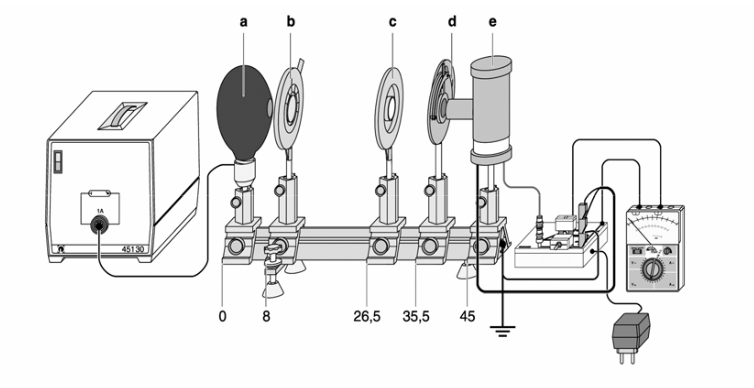
\includegraphics[width=1\linewidth]{imagenes/Captura de pantalla_2023-05-08_13-17-57}
	\caption{Esquema del dispositivo experimental}
	\label{fig:esquema}
\end{figure}
	
	
	Nuestro dispositivo se compone de una lámpara de mercurio de alta presión (a), alimentada por una fuente de alto voltaje; un diafragma (b) para controlar la intensidad de luz; una lente convergente (c) de 100 mm de distancia focal; un revólver (disco giratorio)(d), con diferentes filtros interferenciales de distintas longitudes de onda, de modo que puede rotarse para cambiar el filtro; y una célula fotoeléctrica (e), conectada a un voltímetro (DC) a través de un circuito amplificador externo, donde está el condensador C.
	
	
\begin{figure}[H]
	\centering
	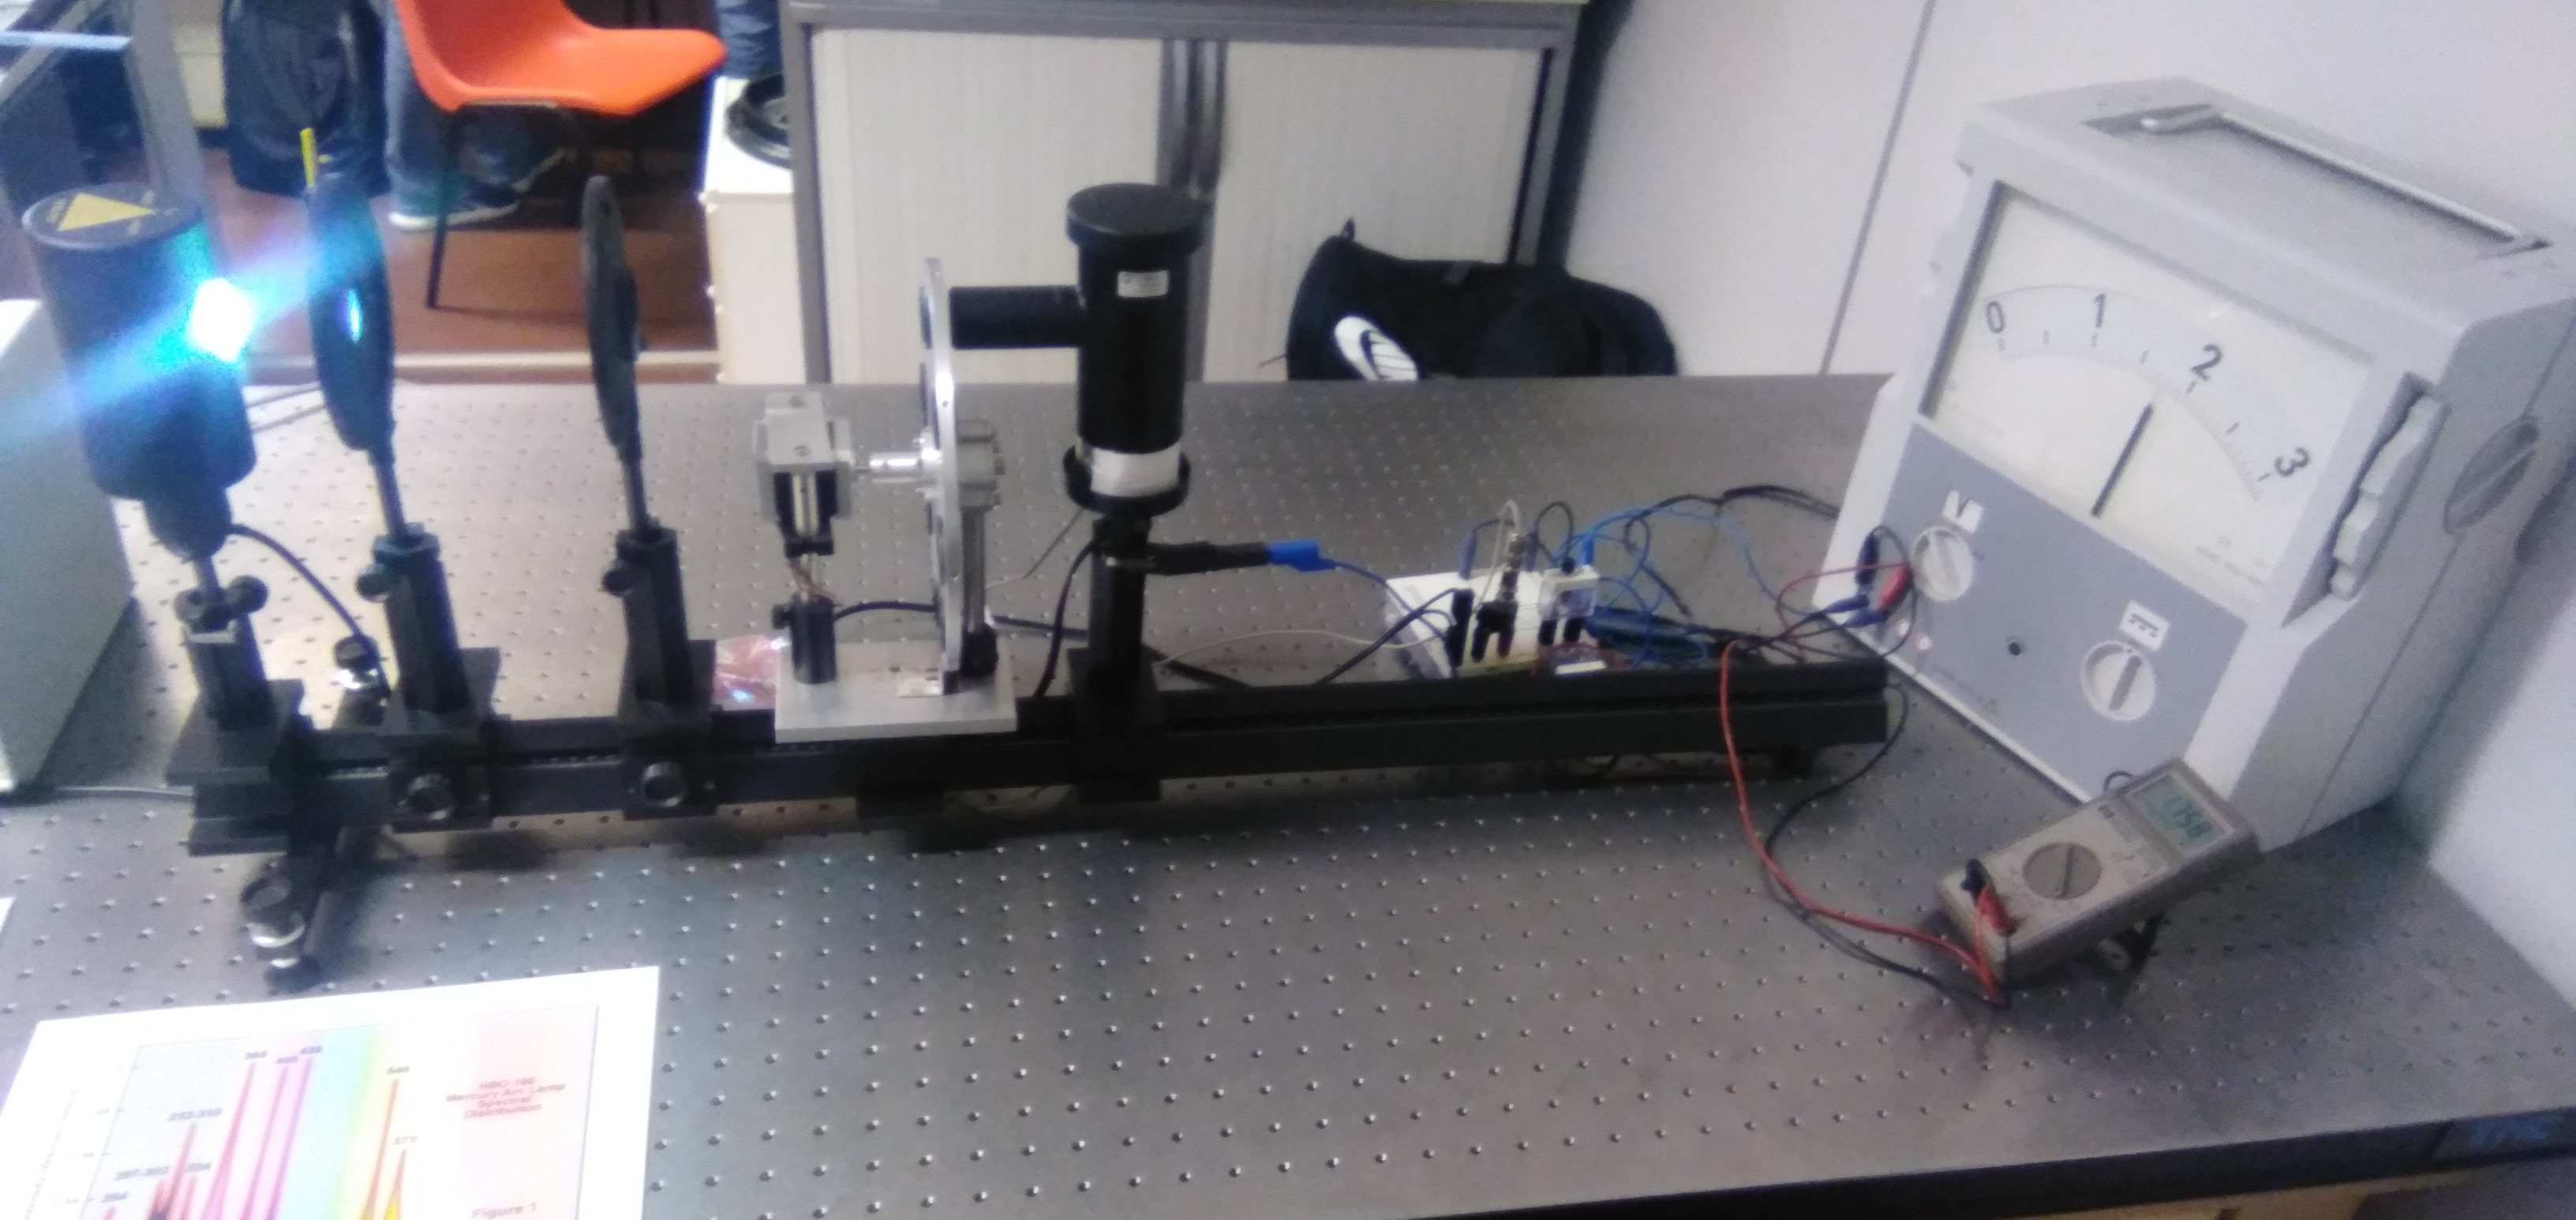
\includegraphics[width=1\linewidth]{imagenes/IMG_20230313_113143_MOD}
	\caption{Fotografía del dispositivo utilizado}
	\label{fig:img20230313113143}
\end{figure}
	
	
	Para cada filtro, tomaremos las medidas del voltaje de frenado indicadas en el voltímetro, y repetiremos esto para dos aberturas distintas del diafragma, de modo que podremos comprobar el efecto de la intensidad en las medidas.
	
	De uno de los filtros se desconoce su longitud de onda, de modo que la deduciremos a partir de la constante de Plank estimada.
	
	Adicionalmente tomaremos una medida con el diafragma casi cerrado, de modo que la intensidad sea mínima, y compararemos con las medidas de otras intensidades.
	
	
	
	
	
	
	
	\section{Tablas de medidas.}
	
	Cada tabla de medidas deberá contener un pie de tabla,
	numerado, donde brevemente se detallen los datos presentados. Cada medida
	deberá ir acompañada de su incertidumbre. Se llevará a cabo el tratamiento de
	incertidumbre de las medidas directas y la propagación de incertidumbre para las
	medidas indirectas. Se añadirán columnas adyacentes que recojan la
	incertidumbre de las magnitudes.
	
	\subsection{Experiencia 1}%: Capacidad calorífica del calorímetro}
	
	\begin{itemize}
		%\centering
		\item Peso vacío: $43,05 \pm 0,01 \si{g}$
		\item $c_{agua}$: $4,18\pm 0,01 \si{Jg^{-1}C^{-1}}$
		%4,1813 \pm 0,0001
	\end{itemize}


\begin{table}[h!]
	\centering
	\begin{tabular}{l|ll|lll|lll|}
		\cline{2-9}
		\textbf{}                               & \multicolumn{2}{l|}{\textbf{TEST 1}}                 & \multicolumn{3}{l|}{\textbf{TEST 2}}                      & \multicolumn{3}{l|}{\textbf{TEST 3}}                      \\ \hline
		\multicolumn{1}{|l|}{\textbf{Dato}}     & \multicolumn{1}{l|}{\textbf{Valor}} & \textbf{Error} & \multicolumn{2}{l|}{\textbf{Valor}} & \textbf{Error}      & \multicolumn{2}{l|}{\textbf{Valor}} & \textbf{Error}      \\ \hline\hline
		\multicolumn{1}{|l|}{$T_i$ (C)}    & \multicolumn{1}{l|}{23,7}           & 0,1           & \multicolumn{2}{l|}{23,0}             & 0,1                & \multicolumn{2}{l|}{22,4}           & 0,1                \\ \hline
		\multicolumn{1}{|l|}{$T_R$ (C)}    & \multicolumn{1}{l|}{0,79}           & 0,01           & \multicolumn{2}{l|}{0,6}            & 0,01                & \multicolumn{2}{l|}{0,62}           & 0,01                \\ \hline
		\multicolumn{1}{|l|}{Peso (g)}     & \multicolumn{1}{l|}{482,33}         & 0,01           & \multicolumn{2}{l|}{482,18}         & 0,01                & \multicolumn{2}{l|}{436,73}         & 0,01                \\ \hline
		\multicolumn{1}{|l|}{$T_{eq}$ (C)} & \multicolumn{1}{l|}{1,4}            & 0,01           & \multicolumn{2}{l|}{1,35}           & 0,01                & \multicolumn{2}{l|}{1,38}           & 0,01                \\ \hline\hline
		\multicolumn{1}{|l|}{$C$ (J/C)}      & \multicolumn{1}{l|}{55,2}           & 1,4            & \multicolumn{2}{l|}{69,8}           & 1,5                 & \multicolumn{2}{l|}{66,0}           & 1,5                 \\ \hline
	\end{tabular}
	\caption{Capacidad calorífica $C$ del calorímetro}
	%\label{tab:my-table}
\end{table}
	
	% $\sigma_{\bar{x}}=\frac{\sigma}{\sqrt{n}}$ % error/desviación en la media
	
	En esta tabla hemos obtenido el valor de $T_{eq}$ observando la temperatura a la que se estabilizaba el sistema agua+calorímetro durante el intercambio, la evolución de la temperatura en el tiempo para las tres pruebas está representada en la Figura \ref{fig:exp1}.
	
	La capacidad calorífica $C$ se obtiene mediante la expresión
	\[ C= \frac{c_{agua}\cdot m_{agua}\cdot(T_{eq}-T_R)}{T_i-T_{eq}}
	\]
	
	siendo $m_{agua}$ la masa de agua correspondiente, calculada restando el peso del calorímetro a su peso en vacío.
	
	El error de $C$ ha sido obtenido mediante propagación de errores:
	
	\[\Delta C = \left|\frac{\partial C}{\partial m}\right|\Delta m + \left|\frac{\partial C}{\partial c}\right|\Delta c + \left|\frac{\partial C}{\partial T_{eq}}\right|\Delta T_{eq} + \left|\frac{\partial C}{\partial T_R}\right|\Delta T_R + \left|\frac{\partial C}{\partial T_i}\right|\Delta T_i\]
	
	Donde $\Delta m$, $\Delta c$, $\Delta T_{eq}$, $\Delta T_R$, y $\Delta T_i$ son las incertidumbres en las mediciones de $m$, $c$, $T_{eq}$, $T_R$, y $T_i$, respectivamente.
	
	Calculando las derivadas parciales correspondientes y sustituyendo estas en la fórmula obtenemos:\\
	
	$\Delta C = \left|\frac{c(T_{eq}-T_R)}{T_i-T_{eq}}\right|\Delta m + \left|\frac{m(T_{eq}-T_R)}{T_i-T_{eq}}\right|\Delta c + \left|\frac{mc}{(T_i-T_{eq})^2} + \frac{m(T_R-T_{eq})}{T_i-T_{eq}}\right|\Delta T_{eq} + \left|\frac{mc}{T_i-T_{eq}}\right|\Delta T_R + \left|\frac{mc(T_{eq}-T_R)}{(T_i-T_{eq})^2}\right|\Delta T_i$
	
	\vspace{12pt}
	\vspace{12pt}
	
	A partir de estos tres valores obtenidos para $C$, podemos obtener la media con su error asociado $\left(\Delta C = \sqrt{\frac{\sum_{i=1}^{n}\Delta C_i^2}{n(n-1)}}  \right)$:
	
	\[\boxed{C = 63,7 \pm 0,9  (\si{J/C}) }\]
	
	\subsection{Experiencia 2}
	
	\begin{itemize}
		%\centering
		\item $m_{agua}$: $460,13 \pm 0,01 \si{g}$
		\item $c_{agua}$: $4,18\pm 0,01 \si{Jg^{-1}C^{-1}}$
	\end{itemize}
	
	
	Tenemos que calcular la capacidad térmica total del calorímetro y la masa de agua introducida mediante:
	\[ C_T = C + m_{agua}\cdot c_{agua}
	\]
	
	y su correspondiente error, que vendrá dado por 
	\[  \Delta C_T = \Delta C + |c_{agua}| \cdot \Delta m_{agua} + |m_{agua}| \cdot \Delta c_{agua}  \]
	
	Obtenemos:
	\[ \boxed{C_T = 1987 \pm 6 \si{J/C}}\]	
	%\[ C_T = 1987 \pm 6 \si{J/C}\]
	
	
	Ahora, a partir de los datos de la temperatura, calcularemos el calor absorbido por el ambiente a lo largo del tiempo, $Q_{amb}$
	
	\[ Q_{amb}(t) = C_T \cdot (T(t)-T_o)
	\]
	
	y su correspondiente error
	
	\[\Delta Q_{amb} = \left|\frac{\partial Q_{amb}}{\partial C_T}\right|\Delta C_T + \left|\frac{\partial Q_{amb}}{\partial T}\right|\Delta T + \left|\frac{\partial Q_{amb}}{\partial T_o}\right|\Delta T_o\]
	
	donde $\Delta C_T$, $\Delta T$ y $\Delta T_o$ son los errores asociados a las variables $C_T$, $T$ y $T_o$ respectivamente. Desarrollando las derivadas parciales:
	
	\[\Delta Q_{amb} = |T-T_o|\cdot\Delta C_T + |C_T|\cdot\Delta T + |-C_T|\cdot\Delta T_o\]
	
	
	Teniendo en cuenta que 
	\begin{itemize}
		%\centering
		\item $  T_o = 0,93\pm 0,01 \text{ºC}  $
		%4,1813 \pm 0,0001
	\end{itemize}
	
	
	
% Please add the following required packages to your document preamble:
% \usepackage[table,xcdraw]{xcolor}
% If you use beamer only pass "xcolor=table" option, i.e. \documentclass[xcolor=table]{beamer}
\begin{table}[H]
	\centering
	\begin{tabular}{|c|c|l|l|l|}
		\hline
		tiempo (s) $\pm 1$ & T (ºC) $\pm 0,01$ & $T-T_o$ & $Q_{amb}$ (J) & $\Delta Q_{amb}$ \\ \hline\hline
		180                & 1,33              & 0,4     & 794,82    & 41,96            \\ \hline
		300                & 1,52              & 0,59    & 1172,36   & 43,01            \\ \hline
		441                & 1,8               & 0,87    & 1728,73   & 44,56            \\ \hline
		476                & 1,85              & 0,92    & 1828,08   & 44,84            \\ \hline
		576                & 2,03              & 1,1     & 2185,75   & 45,83            \\ \hline
		622                & 2,1               & 1,17    & 2324,84   & 46,22            \\ \hline
		722                & 2,29              & 1,36    & 2702,38   & 47,28            \\ \hline
		816                & 2,45              & 1,52    & 3020,31   & 48,16            \\ \hline
		900                & 2,59              & 1,66    & 3298,49   & 48,94            \\ \hline
		916                & 2,6               & 1,67    & 3318,36   & 48,99            \\ \hline
		969                & 2,71              & 1,78    & 3536,94   & 49,60            \\ \hline
		1085               & 2,9               & 1,97    & 3914,48   & 50,65            \\ \hline
		1175               & 3,06              & 2,13    & 4232,40   & 51,54            \\ \hline
		1201               & 3,1               & 2,17    & 4311,88   & 51,76            \\ \hline
		1209               & 3,12              & 2,19    & 4351,63   & 51,87            \\ \hline
		1348               & 3,37              & 2,44    & 4848,39   & 53,26            \\ \hline
		1420               & 3,45              & 2,52    & 5007,35   & 53,70            \\ \hline
		1500               & 3,59              & 2,66    & 5285,54   & 54,48            \\ \hline
		1616               & 3,79              & 2,86    & 5682,94   & 55,59            \\ \hline
		1680               & 3,9               & 2,97    & 5901,52   & 56,19            \\ \hline
		1751               & 4                 & 3,07    & 6100,22   & 56,75            \\ \hline
		1780               & 4,04              & 3,11    & 6179,70   & 56,97            \\ \hline
		1800               & 4,07              & 3,14    & 6239,32   & 57,14            \\ \hline
	\end{tabular}
	\caption{Calor absorbido por el ambiente. Nótese que $Q_{amb}$ y su error están expresados con dos decimales, y no con sus cifras significativas}
	\label{tab:exp2}
\end{table}

Los datos de esta tabla podemos verlos representados en la Figura \ref{fig:exp2}, en la que hemos realizado una regresión lineal que nos permite obtener la tasa de calor absorbida por el ambiente:
\[ q_{amb} = \frac{dQ_{amb}(t)}{dt}
\]

	\subsection{Experiencia 3}

	\begin{itemize}
		%\centering
		\item $m'$: $486,71 \pm 0,01 \si{g}$
		\item $c_{agua}$: $4,18\pm 0,01 \si{Jg^{-1}C^{-1}}$
	\end{itemize}
	

	La nueva capacidad calorífica del sistema será
	\[C_T' = C + m'\cdot c_{agua}
	\] 
	siendo $m'$ la nueva masa de agua.
	Su error, igual que en la sección anterior, 
	\[  \Delta C_T' = \Delta C + |c_{agua}| \cdot \Delta m' + |m'| \cdot \Delta c_{agua}  \]
	
	Por tanto 
	\[  \boxed{ C_T' =  2098 \pm  6 \si{J/C} }\]
	
	Ahora obtendremos el calor absorbido total mediante
	\[ Q_{total}(t) = C_T'\cdot (T(t)-T_o')
	\]
	y su error
	\[\Delta Q_{total} = |T-T_o'|\cdot\Delta C_T' + |C_T'|\cdot\Delta T + |-C_T'|\cdot\Delta T_o'\]
	
	\begin{itemize}
		%\centering
		\item $  T_o' = 3,00\pm 0,01 \text{ºC}  $
		%4,1813 \pm 0,0001
	\end{itemize}

% Please add the following required packages to your document preamble:
% Please add the following required packages to your document preamble:
% \usepackage[table,xcdraw]{xcolor}
% If you use beamer only pass "xcolor=table" option, i.e. \documentclass[xcolor=table]{beamer}
\begin{table}[H]
	\centering
	\begin{tabular}{|c|c|c|c|c|c|c|}
		\hline
		%\rowcolor[HTML]{DAE3F3} 
		\begin{tabular}[c]{@{}l@{}} tiempo(s)\\ $\pm 1$\end{tabular}   &\begin{tabular}[c]{@{}l@{}} $T_{up}$(ºC)\\ $\pm 0,1$\end{tabular} &\begin{tabular}[c]{@{}l@{}} $T_{down}$(ºC)\\ $\pm 0,1$\end{tabular} & \begin{tabular}[c]{@{}l@{}}$T_{agua}$(ºC)\\ $\pm 0,01$\end{tabular} & $T_{up}- T_{down}$ & $Q_{total} $& $\Delta Q_{tot}$ \\ \hline\hline
		20          & 51,5   & 18,3  & 3,3       & 33,2       & 629,44  & 43,71       \\ \hline
		40          & 51,5   & 18,6  & 3,26      & 32,9       & 545,52  & 43,47       \\ \hline
		60          & 51,5   & 19,2  & 3,47      & 32,3       & 986,13  & 44,69       \\ \hline
		80          & 51,5   & 19,2  & 3,67      & 32,3       & 1405,76 & 45,85       \\ \hline
		100         & 51,4   & 19    & 3,81      & 32,4       & 1699,50 & 46,67       \\ \hline
		120         & 51,4   & 19    & 3,97      & 32,4       & 2035,20 & 47,60       \\ \hline
		140         & 51,4   & 19,1  & 4         & 32,3       & 2098,15 & 47,77       \\ \hline
		160         & 51,4   & 19,2  & 4,19      & 32,2       & 2496,80 & 48,88       \\ \hline
		180         & 51,4   & 19,3  & 4,44      & 32,1       & 3021,33 & 50,33       \\ \hline
		200         & 51,5   & 19,1  & 4,54      & 32,4       & 3231,15 & 50,91       \\ \hline
		220         & 51,5   & 19,4  & 4,67      & 32,1       & 3503,91 & 51,66       \\ \hline
		240         & 51,5   & 19,3  & 4,9       & 32,2       & 3986,48 & 53,00       \\ \hline
		260         & 51,5   & 19,4  & 4,91      & 32,1       & 4007,46 & 53,06       \\ \hline
		280         & 51,5   & 19,7  & 5,26      & 31,8       & 4741,81 & 55,09       \\ \hline
		300         & 51,6   & 19,8  & 5,28      & 31,8       & 4783,78 & 55,21       \\ \hline
		320         & 51,6   & 19,9  & 5,56      & 31,7       & 5371,26 & 56,83       \\ \hline
		340         & 51,6   & 19,7  & 5,73      & 31,9       & 5727,94 & 57,82       \\ \hline
		360         & 51,7   & 19,5  & 5,88      & 32,2       & 6042,67 & 58,69       \\ \hline
		380         & 51,7   & 19,3  & 6,04      & 32,4       & 6378,37 & 59,62       \\ \hline
		400         & 51,7   & 19,2  & 6,2       & 32,5       & 6714,07 & 60,55       \\ \hline
	\end{tabular}
	\caption{Calor $Q_{total}$ absorbido por el agua debido a la barra y al ambiente, en función del tiempo. Una vez más el calor y su error representados con dos decimales}
	\label{tab:my-table}
\end{table}
	
	Obtenemos la Figura \ref{fig:exp3}, y de la regresión lineal, su pendiente nos proporciona la tasa de calor absorbida en total:
	\[ q_{total} = \frac{dQ_{total}(t)}{dt}
	\]
	
	
	
	\section{Gráficas.}
	
	
	\iffalse
	Cada gráfica deberá contener un pie de gráfica con una breve
	explicación de la misma. Para cada representación gráfica, se debe incluir en el
	informe una tabla con los datos representados, así como las columnas
	correspondientes a las incertidumbres, ya sean de medidas directas, o por
	propagación de incertidumbres en el caso de medidas indirectas (con esto básicamente tengo que repetir datos pero supongo que tiene sentido). Los ejes de las
	gráficas deben presentar la magnitud representada junto con sus unidades. Elegir
	una escala de los ejes proporcionada respecto al intervalo de datos a representar.
	Cada punto de la gráfica debe mostrar sus correspondientes barras de
	incertidumbre. Cuando se haya realizado un ajuste por mínimos cuadrados de los
	datos, presentar la ecuación de la recta, la incertidumbre de la pendiente y de la
	ordenada en el origen, así como el coeficiente de correlación.
	\fi
	
	
	
	
	\begin{longtable}{|*{12}{c|}}
		 
		
		\hline
		$t_1$ & $\Delta t_1$ & $T_1$ & $\Delta T_1$ & $t_2$ & $\Delta t_2$ & $T_2$ & $\Delta T_2$ & $t_3$ & $\Delta t_3$ & $T_3$ & $\Delta T_3$ \\ \hline \hline
		37 & 1 & 1,55 & 0,01 & 34 & 1 & 1,59 & 0,01 & 36 & 1 & 1,48 & 0,01 \\ \hline 
		38 & 1 & 1,45 & 0,01 & 37 & 1 & 1,45 & 0,01 & 38 & 1 & 1,4 & 0,01 \\ \hline 
		41 & 1 & 1,41 & 0,01 & 39 & 1 & 1,37 & 0,01 & 41 & 1 & 1,37 & 0,01 \\ \hline 
		43 & 1 & 1,38 & 0,01 & 41 & 1 & 1,32 & 0,01 & 43 & 1 & 1,35 & 0,01 \\ \hline 
		46 & 1 & 1,36 & 0,01 & 43 & 1 & 1,29 & 0,01 & 45 & 1 & 1,32 & 0,01 \\ \hline 
		50 & 1 & 1,35 & 0,01 & 45 & 1 & 1,28 & 0,01 & 47 & 1 & 1,29 & 0,01 \\ \hline 
		52 & 1 & 1,33 & 0,01 & 47 & 1 & 1,27 & 0,01 & 49 & 1 & 1,28 & 0,01 \\ \hline 
		55 & 1 & 1,32 & 0,01 & 51 & 1 & 1,27 & 0,01 & 51 & 1 & 1,27 & 0,01 \\ \hline 
		60 & 1 & 1,33 & 0,01 & 53 & 1 & 1,28 & 0,01 & 57 & 1 & 1,27 & 0,01 \\ \hline 
		73 & 1 & 1,32 & 0,01 & 55 & 1 & 1,29 & 0,01 & 59 & 1 & 1,26 & 0,01 \\ \hline 
		76 & 1 & 1,31 & 0,01 & 58 & 1 & 1,31 & 0,01 & 65 & 1 & 1,28 & 0,01 \\ \hline 
		91 & 1 & 1,32 & 0,01 & 62 & 1 & 1,31 & 0,01 & 67 & 1 & 1,31 & 0,01 \\ \hline 
		93 & 1 & 1,33 & 0,01 & 67 & 1 & 1,29 & 0,01 & 69 & 1 & 1,33 & 0,01 \\ \hline 
		94 & 1 & 1,36 & 0,01 & 68 & 1 & 1,28 & 0,01 & 74 & 1 & 1,34 & 0,01 \\ \hline 
		95 & 1 & 1,4 & 0,01 & 73 & 1 & 1,27 & 0,01 & 78 & 1 & 1,35 & 0,01 \\ \hline 
		98 & 1 & 1,44 & 0,01 & 77 & 1 & 1,27 & 0,01 & 85 & 1 & 1,35 & 0,01 \\ \hline 
		100 & 1 & 1,47 & 0,01 & 82 & 1 & 1,28 & 0,01 & 88 & 1 & 1,36 & 0,01 \\ \hline 
		103 & 1 & 1,48 & 0,01 & 84 & 1 & 1,29 & 0,01 & 90 & 1 & 1,37 & 0,01 \\ \hline 
		105 & 1 & 1,49 & 0,01 & 87 & 1 & 1,32 & 0,01 & 92 & 1 & 1,39 & 0,01 \\ \hline 
		107 & 1 & 1,48 & 0,01 & 89 & 1 & 1,33 & 0,01 & 94 & 1 & 1,4 & 0,01 \\ \hline 
		108 & 1 & 1,46 & 0,01 & 92 & 1 & 1,34 & 0,01 & 102 & 1 & 1,39 & 0,01 \\ \hline 
		110 & 1 & 1,45 & 0,01 & 96 & 1 & 1,33 & 0,01 & 115 & 1 & 1,4 & 0,01 \\ \hline 
		112 & 1 & 1,43 & 0,01 & 99 & 1 & 1,32 & 0,01 & 120 & 1 & 1,4 & 0,01 \\ \hline 
		114 & 1 & 1,4 & 0,01 & 104 & 1 & 1,32 & 0,01 & 128 & 1 & 1,39 & 0,01 \\ \hline 
		117 & 1 & 1,39 & 0,01 & 112 & 1 & 1,33 & 0,01 & 131 & 1 & 1,38 & 0,01 \\ \hline 
		119 & 1 & 1,37 & 0,01 & 116 & 1 & 1,34 & 0,01 & 133 & 1 & 1,39 & 0,01 \\ \hline 
		120 & 1 & 1,36 & 0,01 & 119 & 1 & 1,36 & 0,01 & 139 & 1 & 1,4 & 0,01 \\ \hline 
		122 & 1 & 1,35 & 0,01 & 120 & 1 & 1,37 & 0,01 & 145 & 1 & 1,41 & 0,01 \\ \hline 
		124 & 1 & 1,34 & 0,01 & 122 & 1 & 1,38 & 0,01 & 147 & 1 & 1,42 & 0,01 \\ \hline 
		126 & 1 & 1,33 & 0,01 & 125 & 1 & 1,39 & 0,01 & 151 & 1 & 1,43 & 0,01 \\ \hline 
		129 & 1 & 1,32 & 0,01 & 127 & 1 & 1,4 & 0,01 & 154 & 1 & 1,44 & 0,01 \\ \hline 
		133 & 1 & 1,32 & 0,01 & 132 & 1 & 1,39 & 0,01 & 157 & 1 & 1,45 & 0,01 \\ \hline 
		136 & 1 & 1,32 & 0,01 & 138 & 1 & 1,38 & 0,01 & 162 & 1 & 1,46 & 0,01 \\ \hline 
		138 & 1 & 1,31 & 0,01 & 142 & 1 & 1,37 & 0,01 & 164 & 1 & 1,47 & 0,01 \\ \hline 
		142 & 1 & 1,31 & 0,01 & 144 & 1 & 1,36 & 0,01 & 170 & 1 & 1,49 & 0,01 \\ \hline 
		147 & 1 & 1,31 & 0,01 & 149 & 1 & 1,35 & 0,01 & 176 & 1 & 1,5 & 0,01 \\ \hline 
		153 & 1 & 1,32 & 0,01 & 157 & 1 & 1,36 & 0,01 & 178 & 1 & 1,51 & 0,01 \\ \hline 
		155 & 1 & 1,33 & 0,01 & 161 & 1 & 1,37 & 0,01 & 182 & 1 & 1,52 & 0,01 \\ \hline 
		158 & 1 & 1,34 & 0,01 & 164 & 1 & 1,38 & 0,01 & 184 & 1 & 1,53 & 0,01 \\ \hline 
		161 & 1 & 1,34 & 0,01 & 167 & 1 & 1,39 & 0,01 & 186 & 1 & 1,54 & 0,01 \\ \hline 
		164 & 1 & 1,35 & 0,01 & 171 & 1 & 1,41 & 0,01 & 192 & 1 & 1,55 & 0,01 \\ \hline 
		168 & 1 & 1,37 & 0,01 & 177 & 1 & 1,42 & 0,01 & 197 & 1 & 1,56 & 0,01 \\ \hline 
		171 & 1 & 1,37 & 0,01 & 180 & 1 & 1,43 & 0,01 & 203 & 1 & 1,57 & 0,01 \\ \hline 
		175 & 1 & 1,38 & 0,01 & 183 & 1 & 1,44 & 0,01 & 207 & 1 & 1,58 & 0,01 \\ \hline 
		179 & 1 & 1,38 & 0,01 & 185 & 1 & 1,45 & 0,01 & 215 & 1 & 1,59 & 0,01 \\ \hline 
		182 & 1 & 1,39 & 0,01 & 186 & 1 & 1,46 & 0,01 & 217 & 1 & 1,6 & 0,01 \\ \hline 
		188 & 1 & 1,4 & 0,01 & 188 & 1 & 1,47 & 0,01 & 219 & 1 & 1,59 & 0,01 \\ \hline 
		192 & 1 & 1,41 & 0,01 & 196 & 1 & 1,49 & 0,01 & 223 & 1 & 1,6 & 0,01 \\ \hline 
		196 & 1 & 1,42 & 0,01 & 198 & 1 & 1,5 & 0,01 & 229 & 1 & 1,61 & 0,01 \\ \hline 
		199 & 1 & 1,43 & 0,01 & 204 & 1 & 1,51 & 0,01 & 233 & 1 & 1,63 & 0,01 \\ \hline 
		200 & 1 & 1,44 & 0,01 & 206 & 1 & 1,52 & 0,01 &  &  &  &  \\ \hline 
		202 & 1 & 1,45 & 0,01 & 211 & 1 & 1,53 & 0,01 &  &  &  &  \\ \hline 
		206 & 1 & 1,46 & 0,01 &  &  &  &  &  &  &  &  \\ \hline 
		209 & 1 & 1,47 & 0,01 &  &  &  &  &  &  &  &  \\ \hline 
		211 & 1 & 1,48 & 0,01 &  &  &  &  &  &  &  &  \\ \hline 
		214 & 1 & 1,5 & 0,01 &  &  &  &  &  &  &  &  \\ \hline 
		216 & 1 & 1,51 & 0,01 &  &  &  &  &  &  &  &  \\ \hline 
		220 & 1 & 1,52 & 0,01 &  &  &  &  &  &  &  &  \\ \hline 
		224 & 1 & 1,53 & 0,01 &  &  &  &  &  &  &  &  \\ \hline 
		227 & 1 & 1,54 & 0,01 &  &  &  &  &  &  &  &  \\ \hline 
		234 & 1 & 1,55 & 0,01 &  &  &  &  &  &  &  &  \\ \hline 
		237 & 1 & 1,57 & 0,01 &  &  &  &  &  &  &  &  \\ \hline 
		\caption{Datos de la Figura \ref{fig:exp1}}
	\end{longtable} 
	
	
	
	
	
	
	La regresión lineal
	\[f(x) = Ax + B
	\]
	
	siendo 
	\[ A = 3,38 \pm 0,02 \si{J/s}
	\]
	\[B = 230 \pm 20\si{J}
	\]
	
	Coeficiente de determinación: $R^2 = 0,999519196641728$
	 
	%B (y-intercección) = 227,244124065704 +/- 23,2017681590545
	%A (pendiente) = 3,37957175444448 +/- 0,0212936616211874
	%Chi^2 = 12,1171085804928
	%R^2 = 0,999519196641728
	
	
	
	
	
	% Please add the following required packages to your document preamble:
	% \usepackage[table,xcdraw]{xcolor}
	% If you use beamer only pass "xcolor=table" option, i.e. \documentclass[xcolor=table]{beamer}
	\begin{table}[H]
		\centering
		\begin{tabular}{|c|c|l|l|}
			\hline
			tiempo (s)  & Error t & Calor (J)  & Error Q\\ \hline\hline
			180  & 1 & 794,82  & 41,96 \\ \hline
			300  & 1 & 1172,36 & 43,01 \\ \hline
			441  & 1 & 1728,73 & 44,56 \\ \hline
			476  & 1 & 1828,08 & 44,84 \\ \hline
			576  & 1 & 2185,75 & 45,83 \\ \hline
			622  & 1 & 2324,84 & 46,22 \\ \hline
			722  & 1 & 2702,38 & 47,28 \\ \hline
			816  & 1 & 3020,31 & 48,16 \\ \hline
			900  & 1 & 3298,49 & 48,94 \\ \hline
			916  & 1 & 3318,36 & 48,99 \\ \hline
			969  & 1 & 3536,94 & 49,6  \\ \hline
			1085 & 1 & 3914,48 & 50,65 \\ \hline
			1175 & 1 & 4232,4  & 51,54 \\ \hline
			1201 & 1 & 4311,88 & 51,76 \\ \hline
			1209 & 1 & 4351,63 & 51,87 \\ \hline
			1348 & 1 & 4848,39 & 53,26 \\ \hline
			1420 & 1 & 5007,35 & 53,7  \\ \hline
			1500 & 1 & 5285,54 & 54,48 \\ \hline
			1616 & 1 & 5682,94 & 55,59 \\ \hline
			1680 & 1 & 5901,52 & 56,19 \\ \hline
			1751 & 1 & 6100,22 & 56,75 \\ \hline
			1780 & 1 & 6179,7  & 56,97 \\ \hline
			1800 & 1 & 6239,32 & 57,14 \\ \hline
		\end{tabular}
		\caption{Datos de la Figura \ref{fig:exp2}}
		\label{tab:fig2exp2}
	\end{table}
	
	
	

La regresión lineal
\[f(x) = Ax + B
\]

siendo 
\[ A = 16,5 \pm 0,10 \si{J/s}
\]
\[B = 10 \pm 20 \si{J}
\]

Coeficiente de determinación: $R^2 = 0,99432262503481$

%B (y-intercección) = 227,244124065704 +/- 23,2017681590545
%A (pendiente) = 3,37957175444448 +/- 0,0212936616211874
%Chi^2 = 12,1171085804928
%R^2 = 0,99432262503481





% Please add the following required packages to your document preamble:
% \usepackage[table,xcdraw]{xcolor}
% If you use beamer only pass "xcolor=table" option, i.e. \documentclass[xcolor=table]{beamer}
\begin{table}[H]
	\centering
	\begin{tabular}{|c|c|c|c|}
		\hline
		t(s) & Error t & $Q_{tot}$ (J)     & Error $Q_{tot}$ \\ \hline\hline
		%\rowcolor[HTML]{FFFFFF} 
		20   & 1       & 629,44 & 43,71           \\ \hline
		40   & 1       & 545,52            & 43,47           \\ \hline
		60   & 1       & 986,13            & 44,69           \\ \hline
		80   & 1       & 1405,76           & 45,85           \\ \hline
		100  & 1       & 1699,5            & 46,67           \\ \hline
		120  & 1       & 2035,2            & 47,6            \\ \hline
		140  & 1       & 2098,15           & 47,77           \\ \hline
		160  & 1       & 2496,8            & 48,88           \\ \hline
		180  & 1       & 3021,33           & 50,33           \\ \hline
		200  & 1       & 3231,15           & 50,91           \\ \hline
		220  & 1       & 3503,91           & 51,66           \\ \hline
		240  & 1       & 3986,48           & 53              \\ \hline
		260  & 1       & 4007,46           & 53,06           \\ \hline
		280  & 1       & 4741,81           & 55,09           \\ \hline
		300  & 1       & 4783,78           & 55,21           \\ \hline
		320  & 1       & 5371,26           & 56,83           \\ \hline
		340  & 1       & 5727,94           & 57,82           \\ \hline
		360  & 1       & 6042,67           & 58,69           \\ \hline
		380  & 1       & 6378,37           & 59,62           \\ \hline
		400  & 1       & 6714,07           & 60,55           \\ \hline
	\end{tabular}
	\caption{Datos de la Figura \ref{fig:exp3}}
	\label{tab:tab3}
\end{table}


	
	\section{Discusión de resultados.}
	
	\iffalse
	Respuesta razonada a las cuestiones que aparecen en el
	guion de la práctica. Justificación de los resultados. Comparativa de los valores
	experimentales obtenidos con los publicados en la literatura y posibles fuentes de
	incertidumbre en la experimentación que expliquen la discrepancia.
	
	Básicamente comentar los resultados y lo similares que son a lo esperado, comentar las posibles causas de error.
	\fi
	
	A partir de las regresiones de las figuras \ref{fig:exp2} y \ref{fig:exp3} hemos podido obtener que
	\[ q_{amb} = 3,38 \pm 0,02 \si{J/s}
	\]
	\[ q_{total} = 16,5 \pm 0,10\si{J/s}
	\]
	
	Podemos obtener la tasa de calor a través de la barra:
	\[ q_{barra} = q_{total} - q_{amb}
	\]
	y su correspondiente error:
	\[\Delta q_{barra} =\Delta q_{total} + \Delta q_{amb}
	\]
	
	\[\boxed{q_{barra} = 13,12 \pm 0,12 \si{W}}
	\]
	
	Y con ello podemos calcular el valor experimental de la conductividad térmica de la barra:
	\[k_{barra} = \frac{q_{barra}\cdot L}{\Delta T_{barra}\cdot S}
	\]
	siendo su error
	\[\delta k_{barra} = \left|\frac{L}{\Delta T\cdot S}\right|\delta q_{barra} + \left| \frac{q_{barra}}{\Delta T \cdot S} \right|\Delta L +  \left| \frac{-q\cdot L}{\Delta T^2 \cdot S} \right| \delta \Delta T + \left| \frac{-q\cdot L}{\Delta T\cdot S^2} \right| \delta S   \] 
	
	Con los siguiendes datos medidos:
	\begin{itemize}
		\item $L= 0,280 \pm 0,001\si{m}$
		\item $\Delta T_{barra}= 32,2\pm 0,4 \text{K}$
		\item $S = (4,91\pm 0,01)\cdot10^{-4} \si{m^2}$
	\end{itemize}
	
	
	\[ \boxed{k_{barra} = 232 \pm 6  \text{W/( m$\cdot$ K)}     }
	\]
	
	%232,3563269
	
	Según el "Handbook of Chemistry and Physics" (100th Edition, CRC Press, 2019), la conductividad térmica del aluminio es de $237 \text{W/(m·K)}$ a 25ºC, aunque distintas fuentes proporcionan diferentes valores para la conductividad, en el rango de 200 a 240 W/(m·K).
	
	En cualquier caso, la oxidación del aluminio en algunas zonas de la barra es algo que podría causar incertidumbres en la experimentación, aunque no parece ser el caso.
	
	
	\section{Conclusiones.}
	
	\iffalse
	Se incluirá una breve sección de conclusiones donde se expongan las principales conclusiones del estudio.
	
	'' En conclusión hemos visto tal propiedad y comprobado experimentalmente la relación entre tal y cual cosa.''
	
	
	
	\begin{enumerate}
		\item Determinar la capacidad calorífica de un calorímetro a partir de calorimetría de intercambio de calor.
		\item Establecer equilibrios térmicos en calorimetría.
		\item Determinar experimentalmente la conductividad térmica.
	\end{enumerate}
	\fi	
	
	
	En esta práctica hemos realizado el estudio de un sistema térmico con una barra de aluminio y agua en un calorímetro, calculando las tasas de calor absorbido por el ambiente y por el sistema, y hemos podido determinar experimentalmente la conductividad térmica de este aluminio, que ha quedado en torno a los  $237 \text{W/(m·K)}$ que nos indica la literatura.
	
	
	\iffalse
	
	%%%%%%%%%%%%%%%%%%%%%%%%%%%
	\begin{thebibliography}{3}
		%%%%%%%%%%%%%%%%%%%%%%%%%%%
		
		
		% Aquí meter las que corresponda
		
		
		\bibitem{UNED2022} (varios) Guiones de prácticas- Técnicas Experimentales II. Grado en Física. Versión 2.1  UNED, 2022 \url{https://2022.cursosvirtuales.uned.es/o/3754218}
		
		
		\bibitem{UNED2021} (varios) Técnicas Experimentales I. Versión 3.5.  UNED, 2021 \url{https://2021.cursosvirtuales.uned.es/o/42035617}
		
		
		%\bibitem{2021} NOAA National Centers for Environmental Information (NCEI) \url{ https://www.ngdc.noaa.gov/ }
		
	\end{thebibliography}
	\fi
	
	
	
	
	
\end{document}